\chapter{Optimisation du choix de la matrice d'itération}
Nous avons vu dans la partie précédente qu'il existe différentes méthodes pour permettre de résoudre un système linéaire grâce à des méthodes itératives. Ainsi, toujours dans cette idée d'optimisation que nous avons exposé, nous nous sommes posé la question suivante : \og Quelle est la matrice d'itération la plus optimisé pour résoudre un problème \fg. Une méthode est ressortie dans plusieurs ouvrage : Successive Over Relaxation.
\section{Méthode SOR}
C'est dans cette optique que nous nous sommes penchés sur la méthode dite "SOR".
\subsection{Présentation de la méthode SOR}
La méthode SOR (Successive Over Relaxation) est une méthode itérative dérivée de Gauss-Siedel. En effet, le processus de décoposition de la matrice $A$ en deux matrices $M$ et $N$ telles que $A=M-N$ est similaire à l'algorithme de Gauss-Seidel dans la forme des matrices $M$ et $N$.\\

Si la méthode de Gauss-Seidel, vue précédemment, définie la matrice $M$ par $M=D-E$ avec $D$ une matrice diagonale et $E$ une matrice triangulaire inférieure à diagonale nulle et $N=F$, $F$ étant une matrice triangulaire supérieure à diagonale nulle, la méthode SOR définit ses matrices de la manière suivante, en introduisant un paramètre $\omega \in \mathbb{R}^*$ dit de relaxation.
\begin{eqnarray}
M &=& \frac{1}{\omega}D-E\\
N &=& \bigg(\frac{1}{\omega}-1\bigg)D+F
\end{eqnarray}
Par la suite, le procédé est le identique à celui de Gauss-Seidel ou Jacobi et on introduit donc sa matrice d'itération notée $B$.
\begin{equation}
B=M^{-1}N=\bigg[\frac{1}{\omega}D-E\bigg]^{-1}\bigg[\bigg(\frac{1}{\omega}-1\bigg)D+F\bigg]
\end{equation}
On remarquera que si $\omega=1$, on retrouve la méthode de Gauss-Seidel. De plus, si $\omega<1$, on parle de sous-relaxation et de sur-relaxation dans le cas où $\omega>1$.
\subsection{Intérêt de la méthode}
Cette méthode a été développée peu après la Seconde Guerre mondiale afin de proposer une manière de résoudre des systèmes d'équations linéaires, spécifique aux ordinateurs. Si à l'époque, d'autres méthodes avaient été proposées, elles étaient principalement destinées aux êtres humains qui, par des processus non applicables par des ordinateurs, pouvaient assurer la convergence des méthodes. La méthode SOR est donc une méthode qui a fait progresser ce problème en ayant une meilleure vitesse de convergence que les méthodes numériques itératives alors utilisées.\\

L'avantage de la méthode SOR au niveau de la convergence est mathématiquement facilitée par les deux théorèmes suivant:
\begin{enumerate}
	\item \textbf{\underline{Théorème de Kahan (1958)}} : Le rayon spectral de la matrice de relaxation, donnée par :
	$$
	T_\omega=T(\omega)=(I-\omega L)^{-1}{\omega U +(1-\omega)I}
	$$
	vérifie que $\forall \omega \neq 0$,
	$$
	\rho(T_\omega)\geq|\omega -1|
	$$
	\item \textbf{\underline{Théorème d'Ostrowski-Reich (1949-1954)}} : Si la matrice $A$ est définie positive et que $\omega \in ]0;2[$,la méthode SOR converge pour tout choix de vecteur $x^{(0)}$ initial.
\end{enumerate}
Afin qu'une méthode itérative converge, il est nécessaire que le rayon spectral de la matrice d'itération soit strictement inférieur à $1$. Donc, pour que la méthode ne converge pas, il faut que le rayon spectral soit supérieur ou égal à 1. Avec le théorème de Kahan, on a :
$$
|\omega -1|\geq 1 \Leftrightarrow \omega \geq 2 \text{ ou } \omega \leq 0 
$$
Ainsi, nous pouvons déduire du premier théorème, une condition nécessaire non suffisante de la convergence de la méthode SOR qui est :
\begin{equation}
0<\omega<2
\end{equation}
Le deuxième théorème (Ostrowski-Reich), permet quant à lui de conclure par rapport à la convergence de la méthode pour $\omega$ dans l'intervalle $]0;2[$. La combinaison de ces deux théorèmes nous montre que la condition donnée à l'équation $(3.4)$ est nécessaire et, est suffisante dans le cas où $A$ est définie positive.\\

De plus, dans le cas où la matrice $A$ est tridiagonale (les coefficients qui ne sont ni sur la diagonale principale, ni celle au dessus, ni celle au dessous, sont nuls), le théorème suivant nous donne la forme du coefficient de relaxation optimal :\\

Si $A$ est définie positive et est tridiagonale, alors $\rho(T_g)=[\rho(T_j)]^2<1$ et, le choix optimal pour le coefficient de relaxation $\omega$ est donné par : 
$$
\omega_{optimal}=\frac{2}{1+\sqrt{1-[\rho(T_j)]^2}}
$$
Avec ce choix de coefficient de relaxation, on a : $\rho(T_\omega)=\omega-1$\\
La preuve de ce théorème est dans : Ortega, J. M., Numerical
Analysis; A Second Course, Academic Press, New York, 1972, 201 pp.\\
\underline{\textbf{Preuve du théorème de Kahan}} : On a,
$$
\prod\limits_i \lambda_i(T(\omega))=\det(T(\omega))=\frac{\det(\omega U+(1-\omega)I)}{\det(I-\omega L)}=(1-\omega)^n 
$$
Or,
$$
|\prod\limits_i \lambda_i(T(\omega))|\leq\rho(T(\omega))^n \\
\rightarrow |\omega-1|^n\leq\rho(T(\omega))^n\\
$$
Ainsi,
$$
\rho(T(\omega))\geq|\omega-1|
$$
\underline{\textbf{Preuve du théorème d'Ostrowski-Reich}} : En utilisant le théorème de Kahan,on sait qu'il est nécessaire que  $0<\omega<2$ est un critère nécessaire et non suffisant de convergence. De plus, pour une méthode SOR, on a 
$$
M_{SOR}(\omega)+M_{SOR}^*(\omega)-A=\bigg(\frac{2}{\omega-1}\bigg)D \text{ puisque }L=U^*
$$
qui est symétrique définie positive si on est dans l'intervalle donné par le théorème de Kahan. Le théorème de Householder-John nous dit que pour une matrice $A$ hermitienne définie positive, avec $A=M-N$ avec $M$ inversible, la méthode itérative converge pour toute donnée initiale si $M+N^*$ est définie positive. ($N^*$ étant la matrice adjointe ou transconjugée à $N$ soit $N^*=^t\overline{N}=\overline{^tN}$).\\

Afin d'optimiser l'algorithme, on utilise souvent la méthode SSOR (Symetric Successive Over-Relaxation) afin de préconditionner la matrice avant de la traîter, cette méthode sera traîtée ultérieurement dans la partie optimisation.
\subsection{Implémentation numérique}
\section{Les espaces de Krylov}
\subsection{Présentation théorique}
\subsubsection{De Jacobi à Krylov}
On rappelle le résultat de la partie précédente sur la méthode de jacobi qui s'écrit : 
\begin{equation}
x^{k+1} = -D^{-1}(L+U)x^k + D^{-1}b = (I - D^{-1}A)x^{k} + D^{-1}b
\end{equation}
avec la matrice $A$ du système qui se décompose comme : $A = D + L + U$, $L$ une matrice triangulaire inférieur, $U$ un matrice triangulaire supérieur et $D$ diagonale. La matrice A est inversible. On définit ensuite le résidu du système qui est par définition : 
\begin{equation}
r^k \triangleq b - Ax^k = -A ( - A^{-1}b + x^k) = -A (- x^* + x^k)
\end{equation}
Où $x^*$ est la solution réel du système. En normalisant le système ci-dessus de tel sorte que $D = I$. Alors, nous pouvons écrire la solution au rang k+1, comme celle au rang k plus le résidu : 
\begin{eqnarray}
x^{k+1} &=& x^k + r^k\\
\Leftrightarrow x^{k+1} - x^* &=& x^k - x^* + r^k\\
\Leftrightarrow -A( x^{k+1} - x^*) &=& -A(x^k - x^*) - Ar^k\\
\Leftrightarrow r^{k+1} &=& r^k - Ar^k
\end{eqnarray}
Dans cette dernière équation récursive, nous pouvons voir que $r^{k+1}$ est une combinaison linéaire des vecteurs précédents. Ainsi :
\begin{equation}
r^k \in Vect\{r^0, Ar^0, ..., A^kr^0\}
\end{equation}
Cela implique directement : 
\begin{equation}
x^k - x^0 = \sum_{i = 0}^{k-1}r^i
\end{equation}
Donc il vient que : 
\begin{equation}
x^k \in x^0 + Vect\{r^0, Ar^0, ..., A^kr^0\}
\end{equation}
Où $Vect\{r^0, Ar^0, ..., A^kr^0\}$ est le k-ème espace de Krylov généré par A à partir de $r^0$ noté $\mathcal{K}_k(A, r^0)$
\subsubsection{De nouvelles propriétés}
Maintenant que nous avons une définition de ces espaces, nous allons montrer plusieurs propriétés pour ensuite construire l'algorithme afin de l'implémenter. Le premier fait remarquable des espaces de krylov est que par construction, nous avons :  
\begin{equation}
\mathcal{K}_{k - 1}(A, r^0) \in \mathcal{K}_k(A, r^0)
\end{equation}
Ensuite, il est important de montrer que la solution que l'on cherche appartient à cet espace. Nous reprenons donc notre système linéaire possédant une unique solution : 
\begin{equation}
Ax = b \label{pb}
\end{equation}
D'après la définition du problème, la matrice A est inversible. Nous supposons que l'on a le polynôme caractéristique de A :
\begin{equation}
P(\lambda) = \sum_{j = 0}^{n} \alpha_j t^j \Rightarrow P(0) = \alpha_0 = det(A) \neq 0
\end{equation}
Par le théorème de Cayley-Hamilton, nous pouvons obtenir la valeur de $A^{-1}$ :
\begin{eqnarray}
P(A) = \alpha_0 I + \alpha_1 A + ... + \alpha_n A^n &=& 0 \\
\alpha_0 A^{-1}A + \alpha_1 A + ... + \alpha_n A^n &=& 0 \\
(\alpha_0 A^{-1} + \alpha_1  + ... + \alpha_n A^{n - 1})A &=& 0 \\
\alpha_0 A^{-1} + \alpha_1  + ... + \alpha_n A^{n - 1} &=& 0
\end{eqnarray}
Ce qui donne finalement :
\begin{equation}
 A^{-1} = - \frac{1}{\alpha_0} \times \sum_{j=0}^{n-1} \alpha_{j+1} A^j
\end{equation}
Or la solution du problème \ref{pb} est : $x^* = A^{-1}b$. Ce qui peut s'écrire de la façon suivante : 
\begin{equation}
x^* = - \frac{1}{\alpha_0} \sum_{j=0}^{n-1} \alpha_{j+1} A^j b
\end{equation}
Ce vecteur appartient clairement à l'espace de Krylov défini par : 
\begin{equation}
x^* \in \mathcal{K}(A, b)
\end{equation}
Ainsi, la solution de notre problème appartient à l'espace de krylov défini par les deux données du problème que sont A et b. 
\subsection{L'algorithme GMRES}
Un des algorithmes utilisant les espaces de Krylov est l'algorithme GMRES qui se trouve ci-dessous en pseudo-code (cf. figure \ref{fig:gmres}) avec l'implémentation de celui-ci en python.
\begin{figure}
	\centering
	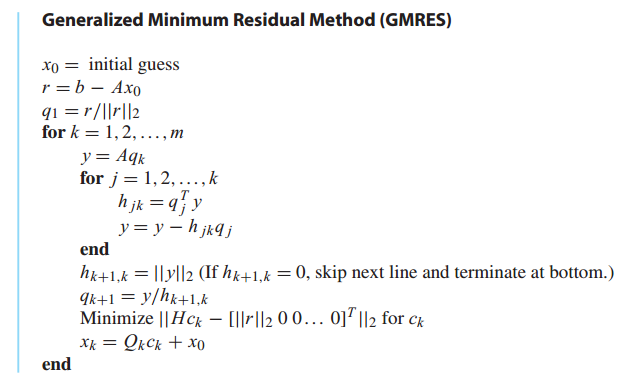
\includegraphics[width=\linewidth]{gmres}
	\caption{Algorithme GMRES}
	\label{fig:gmres}
\end{figure}
\begin{minted}[linenos, autogobble, breaklines]{python}
def GMRES(A, b, espilon):
	max_iter = A.shape[0] #Number of maxiter
	mat_q = np.zeros((max_iter, max_iter + 1))
	mat_h = np.zeros((max_iter + 1, max_iter))
	norm_b = np.linalg.norm(b)
	be1 = np.zeros(max_iter + 1)
	be1[0] = norm_b
	mat_q[:, 0] = 1 / np.linalg.norm(b) * b.T # On définit ici que l'on a forcément x0 = 0
	for j in range(max_iter):
		mat_q[:, j+1] = A @ mat_q[:, j]
		for i in range(j+1):
			mat_h[i, j] = mat_q[:, i] @ mat_q[:, j + 1]
			mat_q[:, j+1] -= mat_h[i, j] * mat_q[:, i]
		mat_h[j + 1, j] = np.linalg.norm(mat_q[:, j + 1])
		mat_q[:, j + 1] /= mat_h[j + 1, j]
		y = np.linalg.lstsq(mat_h, be1, rcond=None)[0]
		residue = np.linalg.norm(y) / norm_b
		if residue < espilon:
			return mat_q[:max_iter, :max_iter] @ y, residue
	return mat_q[:max_iter, :max_iter] @ y
\end{minted}

Cette méthode repose sur les espaces de krylov. En effet, dans cet algorithme nous choisissons $x_k \in \mathcal{K}_k(A, b)$ tel que l'on a $||b - Ax_k||_2$. Nous nous reposons sur une méthode de projection. L'algorithme repose aussi sur le procédé d'Arnoldi qui nous permet de créer une base orthonormal sur le sous-espace de krylov. Dans la suite de ce chapitre, nous allons étudier ces composantes permettant d'arriver à l'écriture de notre algorithme.

\subsubsection{Généralité}

\subsubsection{Procédé d'Arnoldi}

\subsubsection{Explication GMRES}